\documentclass[11pt,a4paper,twoside]{report}
  \usepackage{a4wide}
  \usepackage{epsfig}
  \usepackage{amsmath}
  \usepackage{tabu}
  \usepackage{amsfonts}
  \usepackage{latexsym}
  \usepackage[utf8]{inputenc}
  \usepackage{listings}
  \usepackage{color}
  \usepackage{titlesec}    
  \usepackage{enumitem}
  %\usepackage[catalan]{babel}
  \usepackage{newunicodechar}
  \usepackage{graphicx}
  \usepackage{subcaption}
  \usepackage{float}
  \usepackage[numbered,framed]{matlab-prettifier}
  \usepackage{xcolor}
  \usepackage{pgf, tikz}
  \usepackage{pgfplots}
  \usetikzlibrary{arrows, automata, positioning, datavisualization, datavisualization.formats.functions}
  
\setcounter{tocdepth}{4}
\setcounter{secnumdepth}{4}
  
\newunicodechar{Ŀ}{\L.}
\newunicodechar{ŀ}{\l.}


% \titleformat{\chapter}
%   {\normalfont\LARGE\bfseries}{\thechapter}{1em}{}
% \titlespacing*{\chapter}{0pt}{3.5ex plus 1ex minus .2ex}{2.3ex plus .2ex}

\definecolor{dkgreen}{rgb}{0,0.6,0}
\definecolor{gray}{rgb}{0.5,0.5,0.5}
\definecolor{mauve}{rgb}{0.58,0,0.82}

\lstset{frame=tb,
language=Matlab,
aboveskip=3mm,
belowskip=3mm,
showstringspaces=false,
columns=flexible,
basicstyle={\small\ttfamily},
numbers=none,
numberstyle=\tiny\color{gray},
keywordstyle=\color{blue},
commentstyle=\color{dkgreen},
stringstyle=\color{mauve},
breaklines=true,
breakatwhitespace=true,
tabsize=3,
extendedchars=true,
literate={á}{{\'a}}1 {à}{{\`a}}1 {ã}{{\~a}}1 {é}{{\'e}}1 {è}{{\`e}}1 {í}{{\'i}}1 {ï}{{\"i}}1 {ó}{{\'o}}1 {ò}{{\`o}}1 {ú}{{\'u}}1 {ü}{{\"u}}1 {ç}{{\c{c}}}1
			{Á}{{\'A}}1 {À}{{\`A}}1 {Ã}{{\~A}}1 {É}{{\'E}}1 {È}{{\`E}}1 {Í}{{\'I}}1 {Ï}{{\"I}}1 {Ó}{{\'O}}1 {Ò}{{\`O}}1 {Ú}{{\'U}}1 {Ü}{{\"U}}1 {Ç}{{\c{C}}}1
}


\usepackage{hyperref}
\hypersetup{
  colorlinks=false, %set true if you want colored links
  linktoc=all,     %set to all if you want both sections and subsections linked
  linkcolor=blue,  %choose some color if you want links to stand out
}


\newcommand\double[3][10]{%Passantli A i B genera quatre vertexs virtuals A-B-s, A-B-e (per resepresentar una aresta) i B-A-s, B-A-e (per representar l'altre aresta)
  \draw (#2)
    edge [bend left=#1,draw=none]
    coordinate[at start](#2-#3-s)
    coordinate[at end](#2-#3-e)
    (#3)
    edge [bend right=#1,draw=none]
    coordinate[at start](#3-#2-e)
    coordinate[at end](#3-#2-s)
    (#3);
}

\setlength{\footskip}{50pt}
\setlength{\parindent}{0cm} \setlength{\oddsidemargin}{-0.5cm} \setlength{\evensidemargin}{-0.5cm}
\setlength{\textwidth}{17cm} \setlength{\textheight}{23cm} \setlength{\topmargin}{-1.5cm} \addtolength{\parskip}{2ex}
\setlength{\headsep}{1.5cm}

% "define" Scala
\lstdefinelanguage{scala}{morekeywords={class,object,trait,extends,with,new,if,while,for,def,val,var,this},
otherkeywords={->,=>},
sensitive=true,
morecomment=[l]{//},
morecomment=[s]{/*}{*/},
morestring=[b]"}

% Default settings for code listings
\lstset{frame=tb,language=scala,aboveskip=3mm,belowskip=3mm,showstringspaces=false,columns=flexible,basicstyle={\small\ttfamily}}

\renewcommand{\contentsname}{Continguts}
%\renewcommand{\chaptername}{Pr\`actica}
\setcounter{chapter}{0}

\begin{document}

\title{Pràctica Scala}
\author{Enric Rodriguez, Marc Cané}
\date{29 de novembre de 2018}
\maketitle

\tableofcontents


\chapter{Resultats}

\section{Resultats segons els llindars de simil·litud considerats}

Per comparar els resultats amb diferents llindars hem agafat un nombre de fitxers que contingués suficients documents perquè hi haguessin parelles similars pero alhora no massa gran perquè el càlcul no tardés molt. Hem decidit agafar 300 documents.

La seguent taula mostra el nombre de parelles de documents que obtenim que compleixin cada restricció amb diferents llindars.


\begin{center}
    \begin{tabular}{| c | c | c |}
    \hline
    Llindar & Parells de pàgines similars no interrelacionades & Parells de pàgines no similars interrelacionades \\ \hline 
    0.1 & 127 & 30849 \\ \hline
    0.2 & 24  & 31015 \\ \hline
    0.3 & 7   & 31047 \\ \hline
    0.4 & 4   & 31060 \\ \hline
    0.5 & 2   & 31068 \\
    \hline
    \end{tabular}
\end{center}

A continuació es mostra la sortida de les execucions amb els diferents llindars:
\newline
\newline
\centerline{ \textbf{Llindar = 0.1} }

\textbf{10 primeres parelles de pàgines similars que no es referencien una a l'altra:} \\
William Sholto Douglas, Otto Hoffmann von Waldau -\textgreater 0.1288872009766826 \\
Castell japonès, Ninja -\textgreater 0.24025948403874114 \\ 
William Sholto Douglas, Herbert Otto Gille -\textgreater 0.10360432690191622 \\  
Nantes, William Sholto Douglas -\textgreater 0.10875873369929959 \\ 
William Sholto Douglas, Orde Virtuti Militari -\textgreater 0.16418468360425356 \\  
Copa Volpi per la millor interpretació masculina, Christopher Lee -\textgreater 0.18328534652636125 \\ 
Ofensiva de Prússia Oriental, Front Oriental de la Segona Guerra Mundial -\textgreater 0.3728678286341218 \\ 
William Sholto Douglas, Charles Elwood Yeager -\textgreater 0.1392076132407418 \\ 
Andrew Browne Cunningham, Aleksandr Ivànovitx Pokrixkin -\textgreater 0.11123539067004148 \\ 
Messerschmitt Me 262, Charles Elwood Yeager -\textgreater 0.11234735736587806 \\ 
 \\ 
\textbf{10 primeres parelles de pàgines que es referencien però no són similars:} \\ 
Ruth Benedict, Simfonia núm. 8 (Mahler) -\textgreater 0.009823870046741895 \\ 
Smith, Història de l'Orient Mitjà -\textgreater 0.005021916293628367 \\ 
Sempre en Galiza, Enginyeria inversa -\textgreater 0.0015703616271788405 \\ 
Història de Mali, Palau Reial de Caserta -\textgreater 0.005265578590939846 \\ 
Neonazisme, Corbeta -\textgreater 0.0029017094460869566 \\ 
Memòries d'una geisha (pel·lícula), Reagrupament del Poble Francès -\textgreater 0.005632770711926015 \\ 
Rebecca Clarke, Superheroi -\textgreater 0.005630297770149071 \\ 
Federació Luterana Mundial, Gran Purga -\textgreater 0.0017906154961118467 \\ 
Tres estudis per a figures al peu d'una crucifixió, Història de Kosovo -\textgreater 0.004374072163271377 \\ 
Sivaix, Monarquia -\textgreater 0.00543964030225733 \\ 
 \\ 
\newline
\centerline{ \textbf{Llindar = 0.2} }
\newline
 \\ 
\textbf{10 primeres parelles de pàgines similars que no es referencien una a l'altra:} \\ 
Castell japonès, Ninja -\textgreater 0.24025948403874114 \\ 
Ofensiva de Prússia Oriental, Front Oriental de la Segona Guerra Mundial -\textgreater 0.3728678286341218 \\ 
William Sholto Douglas, Galeazzo Ciano -\textgreater 0.23427707057165204 \\ 
William Sholto Douglas, William Duthie Morgan -\textgreater 0.22460002270186138 \\ 
Romania durant la Segona Guerra Mundial, Carles II de Romania -\textgreater 0.4688662370901408 \\ 
Andrew Browne Cunningham, HMS Illustrious (87) -\textgreater 0.21220274194748687 \\ 
William Sholto Douglas, Andrew McPherson -\textgreater 0.24777401361516543 \\ 
Aleksei Antónov, Vasili Marguèlov -\textgreater 0.2175658681827359 \\ 
Medalla dels Treballadors Distingits, Orde Virtuti Militari -\textgreater 0.22175752010250174 \\ 
Castell japonès, Castell de Malbork -\textgreater 0.20047780310800487 \\ 
 \\ 
\textbf{10 primeres parelles de pàgines que es referencien però no són similars:} \\ 
Ruth Benedict, Simfonia núm. 8 (Mahler) -\textgreater 0.009823870046741895 \\ 
Smith, Història de l'Orient Mitjà -\textgreater 0.005021916293628367 \\ 
Sempre en Galiza, Enginyeria inversa -\textgreater 0.0015703616271788405 \\ 
Història de Mali, Palau Reial de Caserta -\textgreater 0.005265578590939846 \\ 
Neonazisme, Corbeta -\textgreater 0.0029017094460869566 \\ 
Memòries d'una geisha (pel·lícula), Reagrupament del Poble Francès -\textgreater 0.005632770711926015 \\ 
Rebecca Clarke, Superheroi -\textgreater 0.005630297770149071 \\ 
Federació Luterana Mundial, Gran Purga -\textgreater 0.0017906154961118467 \\ 
Tres estudis per a figures al peu d'una crucifixió, Història de Kosovo -\textgreater 0.004374072163271377 \\ 
Sivaix, Monarquia -\textgreater 0.00543964030225733 \\ 
 \\ 
\newline
\centerline{ \textbf{Llindar = 0.3} }
\newline
 \\ 
\textbf{10 primeres parelles de pàgines similars que no es referencien una a l'altra:} \\ 
Ofensiva de Prússia Oriental, Front Oriental de la Segona Guerra Mundial -\textgreater 0.3728678286341218 \\ 
Romania durant la Segona Guerra Mundial, Carles II de Romania -\textgreater 0.4688662370901408 \\ 
Operació Bagration, Ofensiva de Prússia Oriental -\textgreater 0.4248229547539587 \\ 
Batalla del Cap Matapan, HMS Illustrious (87) -\textgreater 0.31551579001078023 \\ 
Història de l'Argentina, Argentina -\textgreater 0.5759558134798274 \\ 
William Sholto Douglas, James O'Meara -\textgreater 0.30860727097192947 \\ 
Fußball-Club Bayern München, Cruzeiro Esporte Clube -\textgreater 0.5139419149640321 \\ 
 \\ 
\textbf{10 primeres parelles de pàgines que es referencien però no són similars:} \\ 
Ruth Benedict, Simfonia núm. 8 (Mahler) -\textgreater 0.009823870046741895 \\ 
Smith, Història de l'Orient Mitjà -\textgreater 0.005021916293628367 \\ 
Sempre en Galiza, Enginyeria inversa -\textgreater 0.0015703616271788405 \\ 
Història de Mali, Palau Reial de Caserta -\textgreater 0.005265578590939846 \\ 
Neonazisme, Corbeta -\textgreater 0.0029017094460869566 \\ 
Memòries d'una geisha (pel·lícula), Reagrupament del Poble Francès -\textgreater 0.005632770711926015 \\ 
Rebecca Clarke, Superheroi -\textgreater 0.005630297770149071 \\ 
Federació Luterana Mundial, Gran Purga -\textgreater 0.0017906154961118467 \\ 
Tres estudis per a figures al peu d'una crucifixió, Història de Kosovo -\textgreater 0.004374072163271377 \\ 
Sivaix, Monarquia -\textgreater 0.00543964030225733 \\ 
 \\ 
\newline
\centerline{ \textbf{Llindar = 0.4} }
\newline
 \\ 
\textbf{10 primeres parelles de pàgines similars que no es referencien una a l'altra:} \\ 
Romania durant la Segona Guerra Mundial, Carles II de Romania -\textgreater 0.4688662370901408 \\ 
Operació Bagration, Ofensiva de Prússia Oriental -\textgreater 0.4248229547539587 \\ 
Història de l'Argentina, Argentina -\textgreater 0.5759558134798274 \\ 
Fußball-Club Bayern München, Cruzeiro Esporte Clube -\textgreater 0.5139419149640321 \\ 
 \\ 
\textbf{10 primeres parelles de pàgines que es referencien però no són similars:} \\ 
Ruth Benedict, Simfonia núm. 8 (Mahler) -\textgreater 0.009823870046741895 \\ 
Smith, Història de l'Orient Mitjà -\textgreater 0.005021916293628367 \\ 
Sempre en Galiza, Enginyeria inversa -\textgreater 0.0015703616271788405 \\ 
Història de Mali, Palau Reial de Caserta -\textgreater 0.005265578590939846 \\ 
Neonazisme, Corbeta -\textgreater 0.0029017094460869566 \\ 
Memòries d'una geisha (pel·lícula), Reagrupament del Poble Francès -\textgreater 0.005632770711926015 \\ 
Rebecca Clarke, Superheroi -\textgreater 0.005630297770149071 \\ 
Federació Luterana Mundial, Gran Purga -\textgreater 0.0017906154961118467 \\ 
Tres estudis per a figures al peu d'una crucifixió, Història de Kosovo -\textgreater 0.004374072163271377 \\ 
Sivaix, Monarquia -\textgreater 0.00543964030225733 \\ 
 \\ 
\newline
\centerline{ \textbf{Llindar = 0.5} }
\newline
 \\ 
\textbf{10 primeres parelles de pàgines similars que no es referencien una a l'altra:} \\ 
Història de l'Argentina, Argentina -\textgreater 0.5759558134798274 \\ 
Fußball-Club Bayern München, Cruzeiro Esporte Clube -\textgreater 0.5139419149640321 \\ 
 \\ 
\textbf{10 primeres parelles de pàgines que es referencien però no són similars:} \\ 
Ruth Benedict, Simfonia núm. 8 (Mahler) -\textgreater 0.009823870046741895 \\ 
Smith, Història de l'Orient Mitjà -\textgreater 0.005021916293628367 \\ 
Sempre en Galiza, Enginyeria inversa -\textgreater 0.0015703616271788405 \\ 
Història de Mali, Palau Reial de Caserta -\textgreater 0.005265578590939846 \\ 
Neonazisme, Corbeta -\textgreater 0.0029017094460869566 \\ 
Memòries d'una geisha (pel·lícula), Reagrupament del Poble Francès -\textgreater 0.005632770711926015 \\ 
Rebecca Clarke, Superheroi -\textgreater 0.005630297770149071 \\ 
Federació Luterana Mundial, Gran Purga -\textgreater 0.0017906154961118467 \\ 
Tres estudis per a figures al peu d'una crucifixió, Història de Kosovo -\textgreater 0.004374072163271377 \\ 
Sivaix, Monarquia -\textgreater 0.00543964030225733 \\

\newpage
\section{Rendiment segons el nombre d'actors en el MapReduce}

Per fer aquestes proves de rendiment hem usat el mètode SecondHalf.MapReduceTfIdf.computeSimilarities(...) amb els 100 primers documents i hem usat el mateix nombre d'actors tant per el $mapper$ com per el $reducer$.


\begin{center}
\begin{tabular}{| c | c | c |}
\hline
Nombre d'actors  & Temps \\ \hline
1  & 23.177229516 \\ \hline
2  & 14.962622731 \\ \hline
3  & 12.921794558 \\ \hline
4  & 12.648637579 \\ \hline
5  & 13.218281647 \\ \hline
8  & 13.171002857 \\ \hline
10 & 12.816006747 \\ \hline
15 & 13.313055689 \\ \hline
20 & 14.519156598 \\ \hline
25 & 15.165376866 \\
\hline
\end{tabular}
\end{center}

Ho podem veure visualment en el seguent gràfic:

\begin{center}
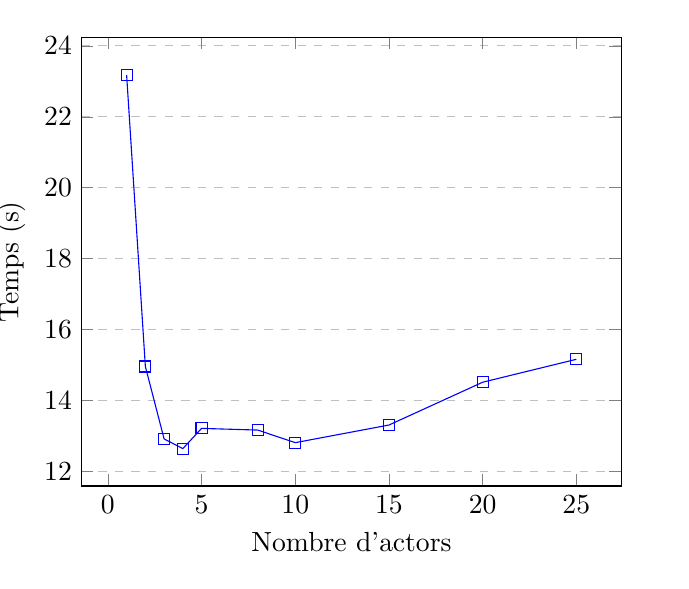
\begin{tikzpicture}
\begin{axis}[
    %title={Gràfic rendiment en funció del nombre d'actors},
    xlabel={Nombre d'actors},
    ylabel={Temps (s)},
    %xmin=0, xmax=100,
    %ymin=0, ymax=120,
    %xtick={0,20,40,60,80,100},
    %ytick={0,20,40,60,80,100,120},
    legend pos=north west,
    ymajorgrids=true,
    grid style=dashed,
]

\addplot[
    color=blue,
    mark=square,
    ]
    coordinates {
    (1, 23.177229516)(2, 14.962622731)(3, 12.921794558)(4, 12.648637579)(5, 13.218281647)(8, 13.171002857)(10, 12.816006747)(15, 13.313055689)(20, 14.519156598)(25, 15.165376866)
    };
 
\end{axis}
\end{tikzpicture}
\end{center}


Les proves de rendiment s'han fet en un intel i5 M430 (2010), 2.26 Ghz, 2 cores, 4 threads, 6 GB de RAM.


\chapter{Exemple de titol}

Quan parlem de matrius disperses ens referim a matrius de grans dimensions en la qual la majoria d'elements son zero. Direm que una matriu és dispersa, quan hi hagi benefici en aplicar els mètodes propis d'aquestes. 

Per identificar si una matriu és dispersa, podem usar el següent:

\qquad Una matriu $n \times n$ serà dispersa si el número de coeficients no nuls es $n^{\gamma+1}$, on $\gamma < 1$.

En funció del problema, decidim el valor del paràmetre $\gamma$. Aquí hi ha els valors típics de $\gamma$:
\begin{itemize}
\item $\gamma=0.2$ per problemes d'anàlisi de sistemes elèctrics de generació i de transport d'energia.
\item $\gamma=0.5$ per matrius en bandes associades a problemes d'anàlisi d'estructures.
\end {itemize}

\chapter{Titol 2}

\section{Per Coordenades}

És la primera aproximació que podríem pensar i és bastant intuïtiva. Per cada element no nul guardem una tupla amb el valor i les seves coordenades: $(a_{i j}, i, j)$. 

A la realitat però, aquest mètode d'emmagatzemar les dades és poc eficient quan hem de fer operacions amb les matrius.

\section{Per files}  
	
També conegut com a \textit{Compressed Sparse Rows (CSR)}, \textit{Compressed Row Storage (CRS)}, o format \textit{Yale}. És el mètode més estès.

Consisteix en guardar els elements ordenats per files, guardar la columna on es troben, i la posició del primer element de cada fila en el vector de valors.
Així ens quedaran tres vectors:
\begin{itemize}
	\item \textbf{valors:} de mida $n_z$, conté tots els valors diferents.
	\item \textbf{columnes:} també de mida $n_z$, conté la columna on es troba cada un dels elements anteriors.
	\item \textbf{iniFiles:} de mida $m+1$, conté la posició on comença cada fila en els vectors valors i columnes, sent $m$ el nombre de files de la matriu. 
\end{itemize}

\subsection{Exemple}

Si es canvien files per columnes, dona la implementació per columnes, o també anomenada \textit{Compressed Sparse Columns (CSC)}.

\subsection{Implementació del mètode CSR}

Hem implementat un script Matlab amb una classe \texttt{CSRSparseMatrix} que guardi les dades necessàries. Aquestes les tenim en ``l'atribut"\texttt{ Matrix} dins del bloc \texttt{properties} (línia 10 del codi següent). Aquestes dades consisteixen en el següent:	
\begin{itemize}
\item  \texttt{Matrix.nColumns}: número de columnes de la matriu, necessari per recrear les files posteriorment.
\item  \texttt{Matrix.values}: vector valors comentat anteriorment, amb els valors no nuls de la matriu.
\item  \texttt{Matrix.columns}: vector de columnes, amb la columna corresponent a cada valor amb el mateix índex.
\item  \texttt{Matrix.beginningRow}: vector amb els índex comença cada fila en el vector de valors i de columnes.
\end{itemize}


\newpage
\section {Codi}

\paragraph*{Exemple codi Scala:}\mbox{}\\

\lstinputlisting[language=Scala]{report_src/exemple.scala}

%\lstinputlisting[language=Scala]{../src/Main.scala}
 
\end{document}
